\documentclass[a4paper, norsk, 12pt]{article}
\usepackage[T1]{fontenc}
\usepackage{fancyvrb}
%\documentclass{article} % was article, thought i'd try with report...
\usepackage{float}
%\usepackage{fullpage} % 1 inch margins
%\usepackage{harvard} % harvard reference style++
\usepackage[hidelinks]{hyperref} % do not remember entirely what this does
%%\usepackage{minted} % [LINUXONLY] list environment with code highlighting
\usepackage[utf8]{inputenc} %To get æøå
\usepackage[norsk]{babel} %Does it norway'ish
%\setcounter{chapter}{-1} %chapter numeration to start on 0
%\usepackage{titlesec} %To make chapter headings different
\usepackage[margin=2.5cm]{geometry}
%\usepackage{longtable} %Table that breakes pages
%\usepackage{tabularx} %Table that breakes lines
\usepackage{ltablex} %Table that combines longtable and tubularx. (Use \begin{tabularx}
\usepackage{graphicx} %To insert image
\usepackage{parskip} %Removes indent and make space between the part sections, like \medskip.
\usepackage[labelformat=empty]{caption} %Removes "Figur 'nr'" in \caption on images.
%\usepackage{color, colortbl} %To use colors in tabulars


\newcommand{\tab}{\hspace*{2em}}

%Removes the indent:
%\setlength\parindent{0pt}

%Changing the paragraph title look:
\makeatletter
\renewcommand\paragraph{\@startsection{paragraph}{4}{\z@}%
  {-3.25ex\@plus -1ex \@minus -.2ex} %To get new line after title
  {1.5ex \@plus .2ex}%
  {\normalfont\large\bfseries}}
\makeatother

%\titleformat{\chapter}[hang]{\bf\huge}{\thechapter}{2pc}{} %To make chapters nice
\title{Oblig 3 \\ IMT3441 \\ Database- og applikasjonsdrift}
\author{Solveig Sørheim 090880 \\ Martin Kristian Mellum 100874}
\date{\today}

%%Useful:
%\hspace*{\fill} \\[-\dimexpr\baselineskip+\parskip\relax] - removes big space after \begin{verbatim}
%\verb - Small kode inline 
%\textt - For bigger kode inline (line breaking)

\begin{document}
\begin{figure}[h!]
 \centering
  
\includegraphics[width=0.5\textwidth]{Images/hig_logo.png}
 %\caption{Bare noko eg skribla på Paint..}
 \maketitle       % make title
\end{figure}
\pagebreak
%%\section{Abstract} % not sure if needed
%%This section is to be written when all else is done. 100-200 words summarizing.
\tableofcontents % make table of contents
\pagebreak	% and break the page, because pretty

\section{Ukesoppgaver - 08. Mars}
\subsection{Oppgave 1}
\subsubsection*{1.1}
Vi undersøkte filen \verb|tf2_50k.dat| i statistikk filen i \verb|LibreOffice|. I statistikk-filen ser vi tabeller med 1\%, 5\% og 10\% frekvenser. I følge oppgavesettet er der 50000 målinger \verb|(tatt hver 5 minutt)| i \verb|tf2_50k.dat| filen.  Målingene viser hvor mange spillere der var i Team Fortress i øyeblikket som var målt. Grafene, dvs de ulike frekvens-tabellene, har forskjellig antall blokker hver. 1\% frekvens har 100 blokker, 5\% har 20 blokker og 10\% har 10 blokker. Størrelsen på blokkene er hvor grov gruppering det er per spillere.\\

Y-aksen i grafene viser antall målinger som er gjort i tusentall.\\
X-aksen representerer antall spillere.\\
En blokk i grafen viser hvor mange målinger som registrerte antall spillere fra sist blokk.\\
Eksempel på 10\% Frekvensgraf:
\begin{itemize}
\item Blokk 1 har   451 på x aksen, og   4 på y aksen.
\item Blokk 2 har 4893 på x aksen, og 26 på y aksen.
\item Blokk 3 har 9336 på x aksen, og 3525 på y aksen.
\end{itemize}

Denne informasjonen viser:
\begin{itemize}
\item Blokk1 hadde 4 målinger som registrerte alt fra 0->451 brukere på disse 4 målingene.
\item Blokk2 hadde 26 målinger som registrerte alt fra 452->4893 brukere på disse 26 målingene.
\item Blokk 3 hadde 3525 målinger, som registrerte alt fra 4894->9336 brukere på disse 3525 målingene.
\end{itemize}

På 10\% grafen teller bolkene antall registreringer av opp til 10\% flere spillere enn max antall spiller registrert, enn den forrige bolken gjorde. \\

Observasjon 10\% statistikk:
\begin{itemize}
\item 4893 spillere - 26 målinger - 0.06%
\item 9336 spillere - 3525 målinger - 7.11%. 
\item 13778 spillere - 15213 målinger - 37.54%
\item 18221 spillere - 16949 målinger - 71.43%
\end{itemize}

Ut ifra denne observasjonen ser vi at observasjon1 målte fra 4894 og opptil 9336 spillere på 3525 målinger, og at der ut ifra dette er 7.11\% sjangse for at der er 9336 eller mindre antall spillere som spiller. Snur vi dette ser vi at det er rundt 93\% sjangse for at der er 9336 eller flere antall spillere som spiller.\\

I observasjon2 ser vi at det er rundt 37.5\% sjangse for at der er 13778 eller mindre antall spillere som spiller, og rundt 63\% sjangse for at der er 13778 eller flere antall spillere som spiller. Og i observasjon3 ser vi at det er rundt 71\% sjangse for at der er 18221 eller mindre antall spillere som spiller, og det er rundt 30\% sjangse for at der er 18221 spillere eller mer som spiller.\\

Under samme tabell, 10\% kategorien, kan vi se at ved å kalibrere serverene til 60\% av det totalt antall målte spillere (27106), ville man hatt nok i 94,73\% av tilfellene. \\

Hvis vi ser på 5\% kategorien vil vi se at det er et hopp ved 70\% av max spillere, der ville man dekket 98.12\% av tilfellene. \\

Hvis vi ser på 1\% kategorien vil se at ved å gå opp til 76\% kapasitet av det som er nødvendig ved maximalt antall spillere vil man dekke 99.05\% av tilfellene. Her ser vi at for å få den siste prosenten dekket må man øke kapasiteten på serverne med 24\%.

\subsubsection*{1.2}
Vi ser ut ifra starten og slutten at det har blitt flere spillere etterhvert. Gjennomsnittet i starten er på 13140, mens det er 18826 spillere i slutten av målinga. I starten er det registrert spillere mellom 7633 og 16581 flest antall ganger, mens i slutten er det registrert mellom 14000 og 24787 spillere flest antall ganger. Det er jevnere målinger i starten og slutten enn det er når man ser på hele målinga.  Man finner ikke de høye toppene i starten og slutten. Det er kanskje fordi spillet ble “Free to play” midt under målinga, og fikk disse voldsomme toppene rundt det. Siden har antall spillere kun økt, dette er vel antageligvis å vente når et spill blir free to play.

\subsubsection*{1.3}
- Vi kan enkelt finne ut hvor mye serverkapasitet som trengs for å la flest mulig brukere vere pålogget samtidig. En kan ut ifra disse målingene da vurdere prosentvis antall brukere man burde ta hensyn til, om det er verdt å bruke mye penger for å ta med de siste prosentene. En kan også enklere vurdere tiltak for disse siste prosentene som da eventuellt ikke blir med i serverkapasiteten.\\

- Man ser ut ifra hvor mange spillere det har vært registrert på det meste, hvor mange spillere man kan “frykte” ved en ny utgivelse, eller oppdatering.\\

- Vi ser at det er en økning i antall spillere fra starten til slutten av målingene, man kan derfor vente seg at dette fortsetter å stige jevnt. Det er derfor er nødvendig å ligge foran det som er behovet i dag, for å kunne klare det økende brukerantallet fremover.


\subsection{Oppgave 2}
\subsubsection*{2.1}
Vi gjorde slik fremgangsmåten i oppgavebeskrivelsen sa. Etter en ti minutters tid fant vi frem til fila og så hva den inneholdte. Dette for å se at ting fungerte.\\

Slik så koden i mysql\_queries ut:
\begin{verbatim}
open(DATA,">>/mysql_queries_long");
my $time = time;
while (<SERVICE>) {
    my ($k, $v) = (m/(\w+).*?(\d+(?:\.\d+)?)/);
    next unless ($k);
    if (exists $WANTED{$k} ) {
        print("$WANTED{$k}.value $v\n");
        print DATA "$time,$WANTED{$k},$v\n";
    }
}
close(DATA);
close(SERVICE);
\end{verbatim}

\subsubsection*{2.2}
Først bestemte vi oss hvordan grafen skulle se ut. Vi kom frem til at grafen skulle inneholde de ulike tallverdiene på venstre side, og 5 minutter på bunnen. I tillegg måtte grafen bare inneholde data fra en av sql verdiene, som insert, select, etc. Dette fordi det er veldig store forskjeller mellom tallverdiene, noen er på tusentall mens andre er på millioner. Vi prøvde så å finne ut hvilken kode vi skulle bruke for å hente ut data fra insert statementen på mysql\_queries\_long. Da kom vi frem til denne koden:

\begin{verbatim}
cat mysql_queries_long | grep insert | cut -d, -f3
\end{verbatim}

Det gav dette resultatet:\\
4674\\
4680\\
4685\\
4689\\
4690\\
4690\\
4690\\
4694\\
4696\\
4697\\
4704\\
4707\\

Logginga ble gjort i 23 timer og tre kvarter, og dekker dermed nesten et helt døgn, noe som gjør det interessant, fordi man ser hvordan ting utvikler seg igjennom døgnet.\\

Vi lagde en fil som inneholdt alle insert spørringene. Deretter prøvde vi å overføre fila til martin sin server ved å bruke denne spørringen:
\begin{verbatim}
scp test.txt ssh martin@kosestua.no:/home/martin/
\end{verbatim}
Det viste seg at vi måtte bruke koda uten ssh.\\

Vi startet Libreoffice og lagde en XY aksis graf der vi la inn insert dataene. Deretter overførte vi resten av spørringene i separate filer til maskinen til Mellum, og la disse inn i andre grafer. Delete og replace hadde under hele logginga 0 antall ganger, derfor lagde vi ikke grafer av dem. Y aksen representerer antall logginger, mens X aksen representerer tid, fordelt på timer. \\

Vedlegget ved er regnearket med grafene for de forskjellige spørringene.

\subsubsection*{2.3}
Vi la inn dataane fra insert.txt inn i det eksisterende regnearket. Her ser vi at de er blitt gjort 278 inserts siden mysql\_query\_long ble opprettet. Da vi startet mysql\_query\_long hadde det allerede blitt gjort 4674 inserts, og etter vi opprettet insert.txt var det blitt gjort 5724 inserts, dvs det har skjedd 1050 inserts på nesten 24 timer. \\

- Forklaring av grafene\\
Grafene viser hvor mange logginger det ble gjort av hver gruppering av verdier. I praksis vil dette si hvor lang tid det tok før det ble gjort et visst antall MySQL spørringer, som var insert i dette tilfelle. Der de høye søylene er ble det med andre ord gjort få spørringer, fordi det er flere logginger av ca. samme antall spørringer. Antall spørringer blir hele tiden også flere, slik at søylene på slutten representerer loggingene som ble gjort på slutten osv. Vi ser ut ifra partiet midt på at det er gjort relativt mange inserts over den perioden, og at det var færre både før og etter. Hvis man teller seg frem for minutter og timer og vet at vi startet loggingen ca. klokka 14:00 så ser man at antall inserts økte rundt midnatt og varte helt til klokka tolv på dagen.

\begin{figure}[h!]
 \centering
  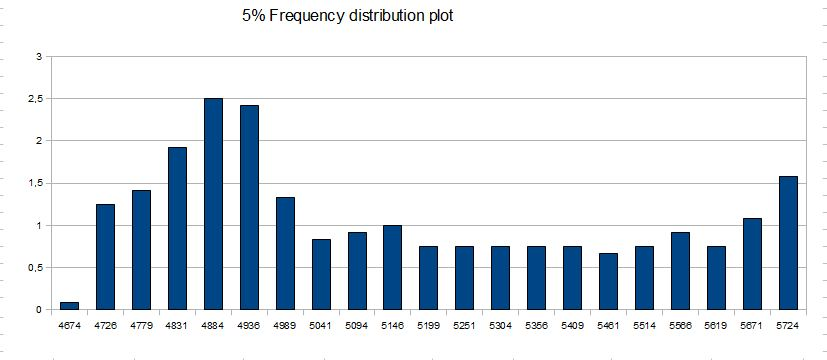
\includegraphics[width=1.0\textwidth]{Images/TF_timer.jpg}
 \caption{Eksempel på omgjøring til timer}
\end{figure}


Vi gjorde om antall logginger til timer, slik at man lettere ser hvor mange timer det tok for hver ca.  50. insert-spørring. Da er det også veldig lett å telle seg frem til hvor i døgnet man er.\\

- Forklaring av tabellene.\\
Vi ser i tabellene at verdien går mellom 4000 og 6000. Percentilen vil i dette tilfelle vise i prosent hvor mange sjekker som har foregått fra og med Rad1 til og med den enkelte raden. Tallet blir basert på det totale antallet sjekker. F.eks:
\begin{itemize}
\item Rad 2: 4779 inserts på 32 sjekker - 11,87 - i 10\% percentile
\item Rad 3: 4884 inserts på 53 sjekker - 30,94 - i 10\% percentile
\item Rad 4: 4989 inserts på 45 sjekker - 47,12 - i 10\% percentile
\end{itemize}

Ut fra disse opplysningene kan vi se at Rad 3 hadde mange flere sjekker enn Rad 2, mens antall inserts er det samme. 10\% percentilen på Rad 3 er 30,94, og dette betyr at rundt 30\% av alle sjekkene skjedde mellom Rad1 og Rad3. Det betyr også at det ble brukt 30\% av hele tidsperioden på mellom Rad1 og Rad3. Dersom vi ser på Rad3 spesifikt, ser vi at denne er 19,07 mer i percentile enn i Rad2. Denne verdien viser at rundt 20\% av alle sjekkene skjedde mellom Rad2 og Rad3, som også betyr at det var veldig lite aktivitet i det tidsrommet frem til neste rad.

\begin{figure}[h!]
 \centering
  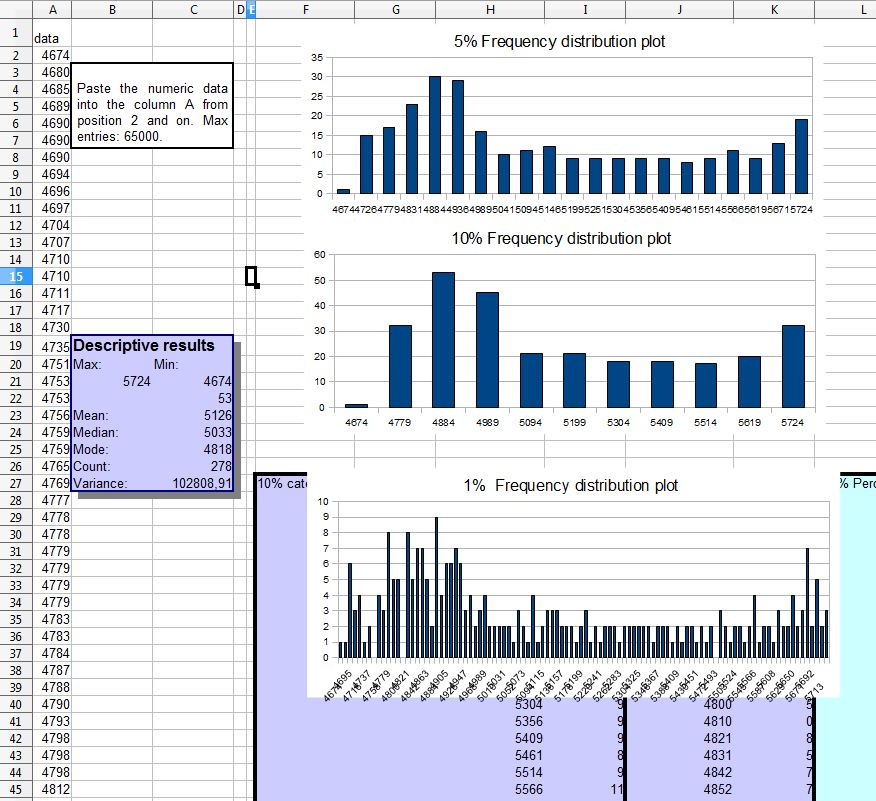
\includegraphics[width=0.8\textwidth]{Images/Insert_i_TF_calc.jpg}
 \caption{Screenshot av dataene}
\end{figure}

\subsection{Oppgave 3}
\subsubsection*{3.1}
Fra mandag til mandag to uker etter så serveren ut til å bruke 5.8 Mb mer trafikk. Om vi tar 100Mb delt på 5.8Mb får vi vite at det vil ta 17.24 to-ukersperioder fær nettet er fylt opp med den samme stigningen man har nå. Ganger man det med to får vi 34.48 uker.

\subsubsection*{3.2}
Forrige oppgave hadde en 100Mb link og fikk 34.5 uker. Dersom vi har en 1Gb link som er 10 ganger så stor, kan vi gange resultatet i forrige oppgave med 10 for å få svaret. Dvs 344,8 uker, eller 6 år og 31 uker.

\subsubsection*{3.3}
Dersom vi følger samme oppsett som 3.1 og 3.2 får vi 3448 uker, eller 66 år og 15 uker.

\subsubsection*{3.4}
Vi antar at disse resultatene er sannsynlige. Det at man sprenger kapasiteten på kun 34.48 uker er noe man må gjøre noe med, dette er alt for nært til at man kan vente med å se hva som skjer.. Hva som skjer seks år eller 66 år frem i tid er ikke den største bekymringa i dag. Da vil all teknologi og nettstandarder være et helt annet sted enn i dag. Noe man derimot bør ha i tankene er hvordan behovet ser ut til å bli om tre år, slik at man har en plan for det. Det at stigningen er linjær gjør at det er lettere å tilpasse seg behovet for nett, fremfor om trafikken gikk i veldige store svingninger uten noe mønster.\\

Man kan se på hvor store f.eks. profilbilder som hele tiden blir vist er. Disse bør ta så liten plass de kan og enda være av grei kvalitet i størrelsen de blir vist i.\\

For å rette problemet kan vi:
\begin{itemize}
\item overvåke
\item skaffe større link
\item teste ytelse (aktiv og passiv)
\end{itemize}

Ytelse foregår ikke bare på applikasjonsnivå, men på veldig mange nivåer helt ned til diskplatene, og alle disse nivåene kan testes på et vis. Nøkkelen til god ytelsesanalyse er å få riktig oversikt over systemets oppførsel. Det er viktig å overvåke om systemet er raskt nok til enhver tid.\\

Der finnes to måter å teste ytelse på: aktiv og passiv. Ved aktiv ytelse går en inn og presser ytelsen til det maksimale. Her finner vi gjerne ekstremverdier som vi ofte ikke ser i vanlig bruk. Passive tester samler derimot reelle data fra vanlig bruk. Der finnes et filsystem, Bonnie++, som bruker systemkall og måler hvor lang tid de tok, som vi kan bruke. Der finnes også andre metoder.

\section{Ukesoppgaver - 15. Mars}
\subsection{Oppgave 1}
Vi la inn mysql og munin-node på db2 samtidig med at vi gjorde dette på db1.

\subsection{Oppgave 2}
Vi fulgte fremgangsmåten i forelesningsfoilen helt til vi skulle endre på my.cnf på db2. Mysql ville ikke starte så lenge linjene som startet med “master” var med. Da vi kommenterte ut de linjene, startet mysql igjen, deretter fulgte vi fremgangsmåten videre uten feil. De linjene gikk bra å ta bort, da vi uansett skreiv det inn i det vi skulle starte slaven.

For å legge inn bf.sql dumpen fra db1 inni den nylagde databasen i db2, prøvde vi på db1 denne kommandoen “cat bf.sql | mysql -u root -p bf -h db2”. Men denne gav feilmelding om at vi ikke har tilgang til db2 fra db1 uten passord. Dermed fant vi ut at vi kunne bruke scp for å overføre sql-filen fra db1 til db2. Dette viste seg å ikke vere enkelt, men vi kom frem til denne koden:
\verb|scp bf.sql root@db2:/home/gruppe7/|

Deretter fulgte vi forelesingsfoileren for å få cat bf.sql inn i bf databasa og videre. Vi hadde tidligere notert ned navnet på binlog-filen og posisjonsnummeret, og brukte det nå. Nå skal vi sjekke om master og slave er synkronisert.

Vi kjørte en \verb|SELECT count(*) FROM user;| på både db1 og db2 å så at begge hadde 2894 users. Deretter gikk vi inn i db1 og gjorde en INSERT for å få inn en user til. Dette slet vi litt med da vi ikke var helt sikre på hvordan vi skulle gjøre med de forskjellige dataene, så det endte med tre flere users enn det vi startet med.

Dette var koden vi brukte for å se hvilke verdier som lå i tabellen user:\\
\verb|mysql -u root -p bf -e "select *, COUNT(*) from posts;"|

Her er en liten del av resultatet som kom:
\begin{verbatim}
postID | userID | text                                  | postDate            | COUNT(*) |
+--------+--------+---------------------------------------+---------------------+----------+
|      1 |     71 | Hillo, ho, ho, boy! Come, bird, come. | 2013-03-01 08:14:35
\end{verbatim}
Så da lagde vi brukere manuelt ved å sette inn en unik userId mm.

Vi gjorde en ny COUNT på db1 og db2, og så at denne også hadde fått tre nye users. Vi konkluderte dermed at databasene var riktig satt opp
\subsection{Oppgave 3}
Vi gjekk inn på db2 og kjørte en count kommando i mysql for å telle antall brukere på slaven. Denne kommandoen er \verb|“select count(*) from user;”|. Antallet som kom frem var 2898. Dermed gjorde vi slave stop på databasen i db2. Deretter gikk vi inn i nettsiden:\\
\verb|128.39.141.231/newuser.php|

Dette gjorde vi et visst antall ganger for å lage nye brukere. Derettet sjekket vi i db1 hvor mange brukere som var der da, og det var 2905 brukere.

Vi gikk inn på db2 igjen å kjørte en COUNT på users kun for å sjekke at det ikke var skjedd noe, vi fikk som ventet samme antall users som før vi stoppa slaven. Deretter startet vi slaven igjen, første COUNT etter starten fikk vi fortsatt det samme antall, mens neste kall vi gjorde fikk vi det oppdaterte antallet ut. Det tok med andre ord kun litt tid før endringene var synkronisert.

Vi konkluderte derfor med at det går fint ann å midlertidig koble slaven fra masteren, og at den vil motta endringer så fort man skrur slaven på igjen.

\subsection{Oppgave 4}
Vi gikk inn på manager og på crontab for å sjekke hvor adressen til backupscriptet lå. Denne lå i backupserveren, (vi lagde denne i oppg 12 i Ukesoppgaver 1.Mars). Deretter gikk vi inni backupserveren og inn i backupscript.sh.

Siden vi allerede hadde satt opp i backupscriptet at vi skulle ta samme type backup av db2 samtidig med backupen av db1 fjernet vi kun linjene som tok backup av db1. Scriptet så slik ut etter dette:
\begin{verbatim}
#!/bin/bash -x
Db2backupfil="backupDb2_$(date +%H_%M_%d_%m).sql"
ssh db2 mysqldump --opt --master-data=2 --flush-logs --all-databases 
-u root -pflee4soda > $Db2backupfil
\end{verbatim}
Vi kjørte backup-scriptet og så at vi kun fikk en ny backup som kom fra db2, og at det var ca. like stor som backupene som tidligere ble tatt av db1 var.
\subsection{Oppgave 5}
Vi gikk inn på \verb|/var/log/mysql| i db1 og brukte cat på \verb|mysql_slow_log| filen. Men her kom det mye tegn som vi tolket som bilder, og vi fikk ingen nyttig informasjon. Så gikk vi inn på \verb|/var/log/mysql| i db2, men der var det ingen \verb|mysql_slow_log| fil. Da gikk vi inn i mysql config filen, og tok vekk kommenteringen på:
\begin{verbatim}
log_slow_queries = /var/log/mysql/mysql-slow.log
long_query_time = 2
\end{verbatim}
Dette ble gjort før påske, og det som følger ble gjort etter:
Vi kom på at det er noe som heter logg-rotering. Vi startet replikering før påske, og logg-rotering skjer på 7 dager. Det vil si at logg-roteringen har slettet filene før replikering skjedde, så vi er ikke i stand til å finne ut om der er noen forskjell på \verb|slow_query| fra tidligere.

\section{Ukesoppgaver - 22. Mars}
\subsection{Oppgave 1}
Vi gjorde som forelesingsnotatene sa, og vi satte av 256 minne i cache.

\subsection{Oppgave 2}
Vi fulgte forelesingsfoilerne og installerte php5-memcache å både www1 og www2 uten problem. 

\subsection{Oppgave 3}
I cache-serveren lastet vi ned \begin{verbatim}memcache_plugins.tar.gz \end{verbatim}på dropbox, og lagde en public link og prøvde å laste den på cache-serveren ved hjelp av denne koden:
\begin{verbatim}
wget https://dl.dropbox.com/u/10542464/memcache_plugins.tar.gz
\end{verbatim}
Men då fikk vi error ved at serveren ikke stolte på serfikatet. Så da søkte vi gjennom manualen til wget etter hvordan vi kunne få maskinen til å laste ned filen selv om han ikke stolte på serfikatet. Da kom vi til denne koden:
\begin{verbatim}
wget --no-check-certificate https://dl.dropbox.com/u/10542464/memcache_plugins.tar.gz
\end{verbatim} 

I cache-maskinen installerte vi perl-memcached biblioteket. Deretter tok vi en apt-get update for å få de siste oppdateringene, og så restartet vi munin-noden.\\

For å ekstraktere tar-filen brukte vi denne koden:

\begin{verbatim}
tar xzf memcache_plugins.tar.gz
\end{verbatim}

Deretter kopierte vi filene, som låg i tar-mappen, over til munin-plugins.\\

I www1 og www2 gikk vi inn i /var/www/config.php og la inn disse linjene: 
\begin{verbatim}
$memcache_enabled = "1";
$memcache_enabled_pictures = "1";
$memcache_server = '10.0.0.7';
\end{verbatim}

Vi restartet apache2 i begge webserverne etter å ha endret config-filen.

\subsection{Oppgave 6}
Etter å ha testet om bookface fungerer ved å skru memcached av og på, konkluderer vi med at bookface fungerer selv om memcached er av eller på.

\subsection{Oppgave 7}
db1 \& db2
\\
Vi ser store forskjeller i mysql-spørringene og nettverkstrafikken i begge serverne. Etter å ha ventet en time etter memcached var satt opp, ser vi at grafene går nedover. 

www1 \& www2
\\
Vi ser at apache-access grafen er noenlunde det samme selv om memcached er slått på. Derimot ser vi store forskjeller i nettverkstrafikk, der trafikken har blitt mye lavere etter at memcached var på.

\subsection{Oppgave 9}
Når memcache var skrudd på fikk vi en load time på 1-2 sekunder.
Når memcache var skrudd av fikk vi mer varierende resultater, alt fra 1 til 8 sekunder.\\

Etter å ha skrudd på igjen memcache fikk vi resultater fra 4 til 8 sekunder. Dette kan konkluderes med at den vil sjekke cache først før den sjekker databasen, og dette tar tid siden i starten får den bare cache misses. Etter det hadde gått noen minutter stabiliserte load timen seg på 1-2 sekunder igjen.

\subsection{Oppgave 10}
Vi fjernet den linjen i config.php som inneheldt \verb|“$memcache_enabled_pictures = "1";”|, og restartet apache i begge webserverne. Etterpå ventet vi i noen minutt og sjekket ved å prøve å kjøre bookface i browseren flere ganger. \\

Noen gangen vart resultatet fra browseren: No connection to database at db1 on port 3306. Mens andre ganger fikk vi opp siden med load time fra 0s til 2s. Grunnen til at load timen er så lav kan vere fordi at nå har memcache plass til mye mer, og bookface blir lastet opp uten bilder først uansett.



%\clearpage
%\addcontentsline{toc}{section}{Referanser} %Add this section to content table
%\bibliographystyle{unsrt} % change for dcu, or something else entirely? unsrt is nice !- referanser
%\bibliography{Referanser}

%\addcontentsline{toc}{section}{Vedlegg} %Add this section to content table
%\section*{Vedlegg}

\end{document}
